%% derived from https://tex.stackexchange.com/questions/357538/graph-of-a-parabola-on-pgfplots
%% Thanks to Stefan Pinnow
%%     https://tex.stackexchange.com/users/95441/stefan-pinnow

  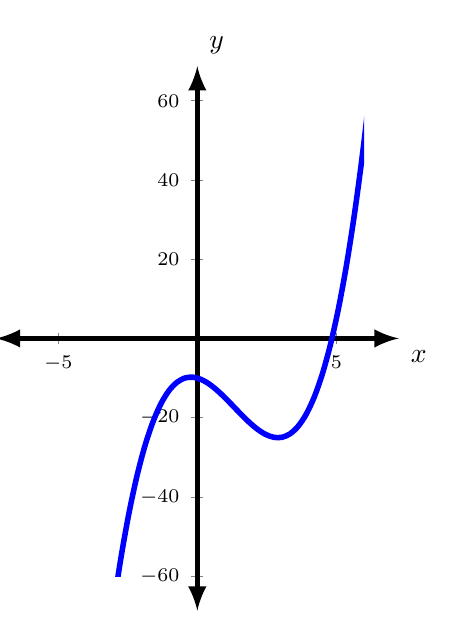
\begin{tikzpicture}[baseline]
    \begin{axis}[
        samples=70,
        smooth,
        domain=-10:10,
        line width=2pt,
        width=0.48\textwidth,
        height=3in,
        axis lines=middle,
        xmin=-6,
        xmax=6,
        ymin=-60,
        ymax=60,
        scaled ticks=false,
        ticklabel style={font=\scriptsize},
        xlabel=$x$,
        ylabel=$y$,
        legend pos=south west,
        legend style={
          anchor=east
        },
        axis line style={
          latex-latex,
          shorten >=-12.5pt,
          shorten <=-12.5pt,
        },
        xlabel style={at={(ticklabel* cs:1)}, xshift=12.5pt, anchor=north west},
        ylabel style={at={(ticklabel* cs:1)}, yshift=12.5pt, anchor=south west},
      ]
      \addplot[color=blue] {x^3 - 4*x^2 - 2*x - 10};
    \end{axis}
  \end{tikzpicture}
